\subsection{Todos/as podem editar?}

Todos/as podem editar a Wikipédia, mas a tarefa não é tão fácil quanto pode parecer. É amplamente documentada a dificuldade de entrada de novos/as editores/as \citep{antin_my_2011}; \citep{burke_feed_2009}; \citep{faulkner_etiquette_2012}; \citep{halfaker_rise_2013}; \citep{kraut_dealing_2010}; \citep{morgan_tea_2013}; \citep{schneider_accept_2014}; \citep{steinmacher_social_2015}. Existem várias regras que dizem o que pode ou não ser escrito, e muitas delas já estão naturalizadas nas ações cotidianas dos/as usuários/as experientes e também nos softwares que gerenciam e atuam na enciclopédia.

Este trabalho pretende pesquisar a aplicação destas regras, entendendo seu histórico de criação, seu processo de naturalização e os efeitos que causam nos/as novatos/as que são pegos/as de surpresa ao tentar editar, e não tem ideia de todo o complexo mundo de governança da enciclopédia.

A Wikipédia é o décimo site mais acessado do mundo, e o décimo-quinto do Brasil. Em ambos os rankings é o site mais visitado mantido por uma instituição sem fins lucrativos \citep{alexa_2019}. No ano de 2019, apresentou uma média de 500 milhões de visitantes únicos por mês \citep{wikimedia_stats_2019}. Os imponentes números de sua audiência dizem que uma informação que perdure na Wikipédia tenderá a ser lida por milhares de pessoas e replicada indefinidamente, o que nos mostra a grande relevância desta ferramenta no mundo contemporâneo e sua centralidade na construção de fatos em nosso tempo.

Todos esses acessos estão distribuídos entre mais de 40 milhões de verbetes escritos em diferentes 303 idiomas, que atualmente são mantidos por aproximadamente 400 mil editores/as ativos/as \citep{wikimedia_stats_2019}. No momento, a versão lusófona conta com um pouco mais de um milhão de verbetes, mantidos por aproximadamente 3600 usuários/as ativos/as \citep{wikimedia_stats_2020}\footnote{Dados encontrados em https://stats.wikimedia.org/\#/pt.wikipedia.org/contributing/active-editors/normal|line|2-year|~total|monthly , acessada em 12/02/2020.}. É inquestionável que seus números de editores são grandiosos, e a um primeiro olhar esse volume pode parecer sustentar a afirmação de que afinal "\textit{qualquer um/a pode editar}".

A primeira cena apresentada versa sobre Jimmy Wales, um dos fundadores da Wikipédia e diretor executivo da Wikimedia Foundation até 2007. Ao contrário do que se poderia achar, sua saída da fundação, há mais de uma década, não fez desaparecer o discurso aqui posto à prova pelas cenas. Sua sucessora, Sue Gardner, manteve a linha do discurso, como pode ser visto em diversas falas\footnote{Publicação feita em seu blog pessoal acessada em 12/02/2020. https://suegardner.org/2013/01/14/the-people-behind-wikipedia-the-encyclopedia-anyone-can-edit/ .}, palestras\footnote{Palestra apresentada em 2010 e acessada em 12/02/2020 https://www.youtube.com/watch?v=vzJCHQ42XAw\&t=127s .} e entrevistas\footnote{Entrevista concedida em 2013 e acessada em 12/02/2020 https://www.youtube.com/watch?v=Y6gYhHWglBA .} concedidas ao longo dos 8 anos de sua gestão. Gestão marcada pela construção de programas que buscaram estimular a contribuição editorial de grupos sociais sub representados dentre os/as editores/as da enciclopédia, tais como moradores/as do sul global e mulheres, levantando uma bandeira que podemos tentar resumir em "todos/as devem ter condições de editar"\footnote{Esse discurso pode ser encontrado em diversos materiais, tais como esta entrevista dada em 2012 e acessada em 12/02/2020 https://www.youtube.com/watch?v=UoWgqPcF-TQ .}, mas sem jamais abandonar o "qualquer um/a pode editar".

A expressão "qualquer um/a pode editar a Wikipédia"\footnote{A expressão utilizada no buscador foi exatamente: "qualquer um pode editar" Wikipédia} é tão onipresente em discursos de \textit{hackers}, militantes da cultura livre, professores/as e até mesmo de seus/suas críticos/as que, uma rápida busca por ela no Google, retorna mais de 18 mil resultados. Indo além, ao testarmos a versão original da afirmação em inglês “\textit{anyone can edit Wikipedia}”\footnote{A expressão utilizada no buscador foi exatamente: "anyone can edit" Wikipedia}, a maior ferramenta de buscas do mercado retornou mais de 660 mil links\footnote{Buscas realizadas no endereço www.google.com em 28/01/2020.}.

Fazendo um recorte apenas por trabalhos acadêmicos, utilizando a ferramenta Google Scholar\footnote{Busca realizada no serviço https://scholar.google.com em 28/01/2020.}, nos foram apresentados mais de 3 mil trabalhos com o referido termo em inglês. Esse enorme volume sustenta que nossa cena inaugural não está descolada da realidade, e reforça a popularidade do termo, inclusive dentre os/as estudiosos/as da enciclopédia virtual.

É importante notar que o discurso está presente tanto na fala dos/as defensores/as do modelo distribuído da enciclopédia como na de seus/suas críticos/as. O que para alguns é visto como um diferencial competitivo, para outros é um problema irreparável. Não é difícil encontrar tanto falas de intelectuais como expressões da cultura popular do mundo digital contemporâneo, através dos memes\footnote{Diversos exemplos de memes podem ser encontrados em buscas como https://www.google.com/search?q=meme+wikipedia+anyone+can+edit\&tbm=isch. Nos exemplos aqui exibidos na figura \ref{fig:memes}, a primeira imagem está escrito sobre a vítima ``Usando Wikipédia como fonte'' e sobre o atirador ``Mas qualquer um pode editar''. Segunda imagem: acima da professora está escrito ``Você não pode utilizar a Wikipédia como fonte'', e abaixo "qualquer um pode editar".}, atacando a Wikipédia exatamente por qualquer um poder editá-la. A própria Wikipédia mantém um verbete chamado ``Críticas à Wikipédia'', e dos seus 39 tópicos, o primeiro a ser apresentado é não por acaso chamado ``Crítica ao conteúdo'', que apresenta um texto de Robert McHenry, editor da Encyclopædia Britannica, afirmando não ser possível existir a fiabilidade enciclopédica em uma obra editável abertamente. \citewiki{ptwiki_criticas}\footnote{Sempre que uma página de uma Wikipédia for citada durante o estudo ela será referenciada seguindo o padrão: (``idioma'', ``nome da página'', ``data da edição'').}

\begin{figure}[H]
    \centering
    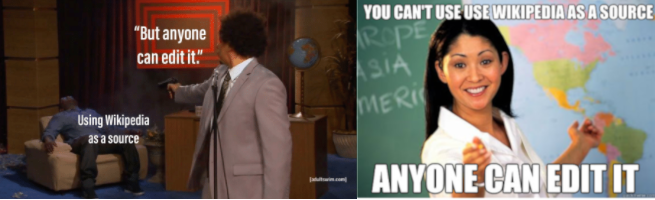
\includegraphics[width=1\textwidth]{Images/memes.png}
    \caption{Exemplos de memes sobre a Wikipédia.}
    \label{fig:memes}
\end{figure}

Os questionamentos de críticos relacionados a impossibilidade de se manter uma enciclopédia de qualidade que "qualquer um/a possa editar" são recorrentemente explorados e discutidos por professores/as, conteudistas, jornalistas e pesquisadores/as. Nestes questionamentos diversos fatores são colocados em xeque, mas invariavelmente todos assumem como verdade a afirmação de que "qualquer um/a pode editar". Não encontramos na literatura esforços para testar esta assertiva, esmiuçando o discurso propagado por todos os lados, sustentado em seus grandiosos números globais e na estrutura de uma ferramenta wiki aberta e colaborativa.

Assim, iremos nas próximas seções iniciar esforços de verificação na prática cotidiana, na vida real dos ``qualquer uns/umas'', a consistência deste discurso.